\documentclass[12pt]{article}
\usepackage{color}
\usepackage{tikz, pgfplots}
\usetikzlibrary{arrows.meta, calc, positioning}
\usetikzlibrary{decorations.pathmorphing}
\usepackage{amsmath}
\usepackage[utf8]{inputenc}
\usepackage[
      colorlinks=true,
      linkcolor=red,
      urlcolor=red,
      filecolor=black,
      citecolor=red,
      ]{hyperref}

\begin{document}

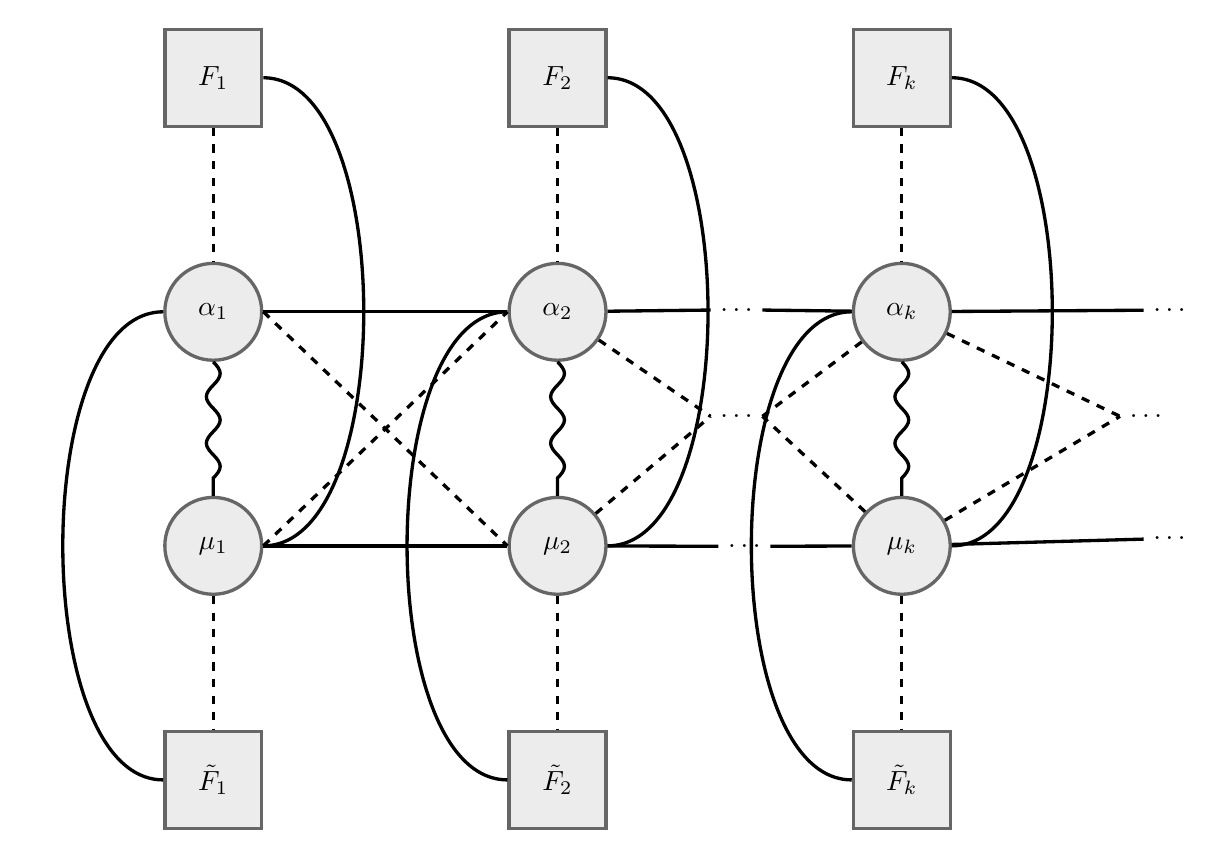
\begin{tikzpicture}
[
node distance = 17mm and 31mm,
b/.style={rectangle, draw=black!60, fill=gray!15, very thick, minimum size=35},
c/.style={circle, draw=black!60, fill=gray!15, very thick, minimum size=35}
]

%Nodes
\node[b]      (posFk)                            	{$F_k$};
\node[c]      (posak)      [below=of posFk]     	{$\alpha_k$};
\node[c]      (posmuk)     [below=of posak]      	{$\mu_k$};
\node[b]      (posFtk)     [below=of posmuk]      {$\tilde{F}_k$};

\node[b]      (posFF)      [left=of posFk]      	{$F_2$};
\node[c]      (posakk)     [below=of posFF]      	{$\alpha_2$};
\node[c]      (posmukk)    [below=of posakk]      {$\mu_2$};
\node[b]      (posFtkk)    [below=of posmukk]     {$\tilde{F}_2$};

\node[b]      (posFFF)     [left=of posFF]      	{$F_1$};
\node[c]      (posakkk)    [below=of posFFF]     	{$\alpha_1$};
\node[c]      (posmukkk)   [below=of posakkk]     {$\mu_1$};
\node[b]      (posFtkkk)   [below=of posmukkk]    {$\tilde{F}_1$};

%Curved lines for the quiver
\draw[-, very thick] (posmuk.east) 	.. controls  +(right:17mm) and +(right:17mm)   	.. (posFk.east);
\draw[-, very thick] (posak.west) 		.. controls  +(left:17mm) and +(left:17mm)   		.. (posFtk.west);
\draw[-, very thick] (posmukk.east) 	.. controls  +(right:17mm) and +(right:17mm)   	.. (posFF.east);
\draw[-, very thick] (posakk.west) 	.. controls  +(left:17mm) and +(left:17mm)   		.. (posFtkk.west);
\draw[-, very thick] (posmukkk.east) 	.. controls  +(right:17mm) and +(right:17mm)   	.. (posFFF.east);
\draw[-, very thick] (posakkk.west) 	.. controls  +(left:17mm) and +(left:17mm)   		.. (posFtkkk.west);

%Lines for each column of the quivers
%Right
\draw[-, very thick, dashed] (posFk.south)  														to node[right] {} (posak.north);
\draw[-, very thick, decorate,decoration={coil,aspect=0,segment length=5.9mm}] (posak.south)  	to node[right] {} (posmuk.north);
\draw[-, very thick, dashed] (posmuk.south)  														to node[right] {} (posFtk.north);

%Middle
\draw[-, very thick, dashed] (posFF.south)  														to node[right] {} (posakk.north);
\draw[-, very thick, decorate,decoration={coil,aspect=0,segment length=5.9mm}] (posakk.south)  	to node[right] {} (posmukk.north);
\draw[-, very thick, dashed] (posmukk.south)  													to node[right] {} (posFtkk.north);

%Left
\draw[-, very thick, dashed] (posFFF.south)  														to node[right] {} (posakkk.north);
\draw[-, very thick, decorate,decoration={coil,aspect=0,segment length=5.9mm}] (posakkk.south) 	to node[right] {} (posmukkk.north);
\draw[-, very thick, dashed] (posmukkk.south)  													to node[right] {} (posFtkkk.north);

%Horizontal lines connecting the quiver
\draw[-, very thick] (posakkk.east)  	to node[right] {} (posakk.west);
\draw[-, very thick] (posmukkk.east)  to node[right] {} (posmukk.west);

%Diagonal lines connecting the first part of the quiver
\draw[-, very thick, dashed] (posakkk.east)  	to node[right] {} (posmukk.west);
\draw[-, very thick, dashed] (posmukkk.east)  to node[right] {} (posakk.west);

%Finishing off the middle part of the quiver
\node at (31mm,-43mm) (aux0) {$\bf\textcolor{black}{\ldots}$};
\draw[-, very thick, dashed] (posak) to node[right] {} (aux0.west);
\draw[-, very thick, dashed] (posmuk) to node[right] {} (aux0.west);

%Finishing off the straight lines
\node at (34mm,-29.5mm) (aux1) {$\bf\textcolor{black}{\ldots}$};
\node at (34mm,-58.5mm) (aux2) {$\bf\textcolor{black}{\ldots}$};
\draw[-, very thick]  (posak) to node[right] {} (aux1);
\draw[-, very thick] (posmuk) to node[right] {} (aux2);

%Connecting the middle part of the quiver diagram
\node at (-21mm,-43mm) (aux3) {$\bf\textcolor{black}{\ldots}$};
\draw[-, very thick, dashed] (posakk) to node[right] {} (aux3.west);
\draw[-, very thick, dashed] (posmukk) to node[right] {} (aux3.west);
\draw[-, very thick, dashed] (posak) to node[left] {} (aux3.east);
\draw[-, very thick, dashed] (posmuk) to node[left] {} (aux3.east);
\node at (-21mm,-29.5mm) (aux4) {$\bf\textcolor{black}{\ldots}$};
\draw[-, very thick] (posakk) to node[right] {} (aux4.west);
\draw[-, very thick] (posak) to node[left] {} (aux4.east);
\node at (-20mm,-59.5mm) (aux5) {$\bf\textcolor{black}{\ldots}$};
\draw[-, very thick] (posmukk) to node[right] {} (aux5.west);
\draw[-, very thick] (posmuk) to node[left] {} (aux5.east);

\end{tikzpicture}

\end{document}